\newpage
\section{Analiza danych}
W tym rozdziale zostaną pokazane wyniki analizy zebranych danych. Zostaną zbadane podstawowe charakterystyki kont, publikowanych przez nie postów oraz użytkowników będących ich odbiorcami.  Celem tych działań jest zbadanie istniejących właściwości klas kont oraz znalezienie zależności lub różnic pomiędzy nimi.  
\subsection{Liczba followersów }Dla konta o największej ilości followersów została utworzona osobna kategoria o\,nazwie Bigmainstream. Stało się tak ponieważ, gazeta\_pl, która posiada najmniej followersów z\,tej dodatkowej kategorii i\,tak posiada ponad 3 razy tyle followersów niż kolejne najbardziej popularne konto jakim jest rzeczpospolita.
\begin{figure}[!h]
	\label{fig:followers}
	\centering 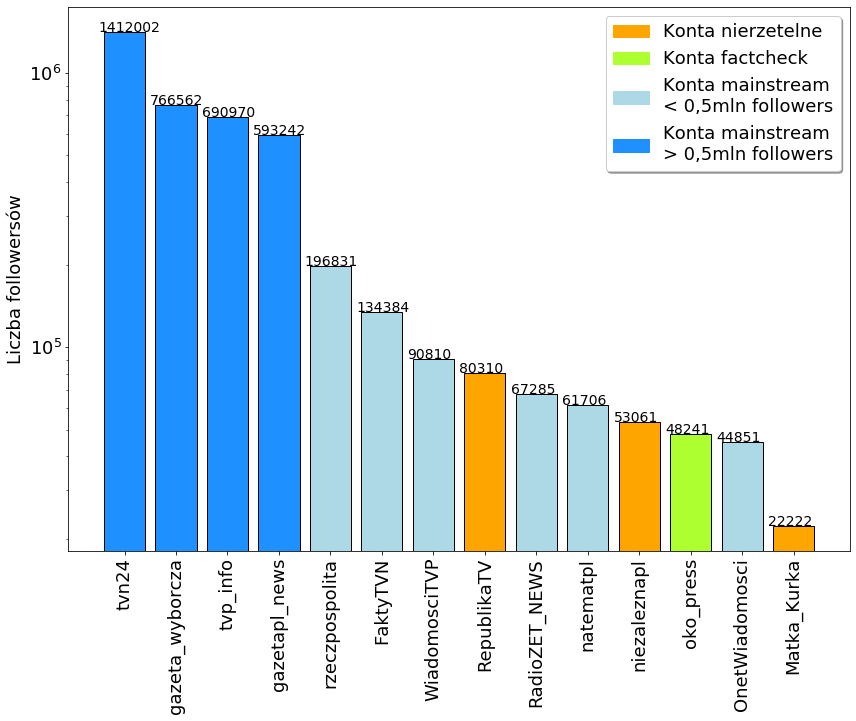
\includegraphics[width=0.9\linewidth]{img/results/followers.png}
	\caption{Wykres liczby followersów najbardziej popularnych kont z\,podziałem na przynależność do klasy}
\end{figure}
\par
W pierwszej dziesiątce najpopularniejszych kont z\,przeprowadzanej analizy (z wyłączeniem Bigmainstream) trzy pozycje zajmują konta oznaczone jako Junk. Z\,tej kategorii najwięcej followersów ma RepublikaTV i\,znajduje się ona na 4 miejscu. Strona z\,kategorii Factcheck znalazła się dopiero na siódmym miejscu w\,popularności.

\subsection{Liczba tweetów}
Konta mediów zakwalifikowanych jako mainstreamowe łącznie opublikowały łącznie 25 tysięcy postów, w\,tym 8 tysięcy postów należy do kont posiadających ponad pół miliona followersów. Natomiast konta Junk opublikowały 10 tysięcy postów. W\,te statystyki wliczają się tweety oryginalnie opublikowane przez te konta jak i\,udostępnione przez nie retweety.  
\par
Sprawdzono, jak duża część zebranych tweetów w\,każdej klasie jest oryginalnie stworzona przez znajdujące się w\,niej konta. Wyniki przedstawiono w\,tabeli \ref{tab:liczbatweetowklasy}. Okazuje się, że największy procent oryginalnych tweetów do wszystkich tweetów publikują konta z\,klasy Nierzetelne. Natomiast najmniej, bo tylko 75\% tweetów publikowanych przez konta mainstream, jest oryginalnie przez nie postowany.
\begin{table}[!h]
\centering 
\caption{Porównanie liczby oryginalnych tweetów do wszystkich tweetów danej klasy.} \label{tab:liczbatweetowklasy}
\begin{tabular}{|m{2,8cm}|R{2,5cm}|R{2,5cm}|R{2,5cm}|R{2,5cm}|} 
\hline
~Klasa & Suma 
  wszystkich & Suma 
  \mbox{oryginalnych} & Procent
  
  oryginalnych & Średnia
  
  oryginalnych
  /dzień \\ 
\hline
NIERZETELNE & 10466 & 10246 & 98\% & 330.5 \\ 
\hline
MAINSTREAM \textless{}
  0,5 mln & 17484 & 12566 & 72\% & 405.4 \\ 
\hline
MAINSTREAM \textgreater{}
  0,5mln & 8078 & 6463 & 80\% & 208.5 \\ 
\hline
FACTCHECK & 644 & 607 & 94\% & 19.6 \\
\hline
\end{tabular}
\end{table}

\subsection{Analiza aktywności kont}
Posiadając informacje na temat oryginalnych tweetów, można było zbadać z\,jak duzo nowych tweetów jest publikowane przez konta w\,każdej klasie. Ogólne dane przedstawiono w\,tabeli \ref{tab:liczbatweetowklasy}. W\,tym przypadku dla lepszego rozeznania zdecydowano się spojrzeć które konta są najbardziej aktywne. Może się bowiem zdarzyć, że w\,zbiorze kont, tylko kilka z\,nich publikuje bardzo duzo treści natomiast inne ograniczają liczbę swoich publikacji. 
\par
\begin{figure}[!h]
	\centering 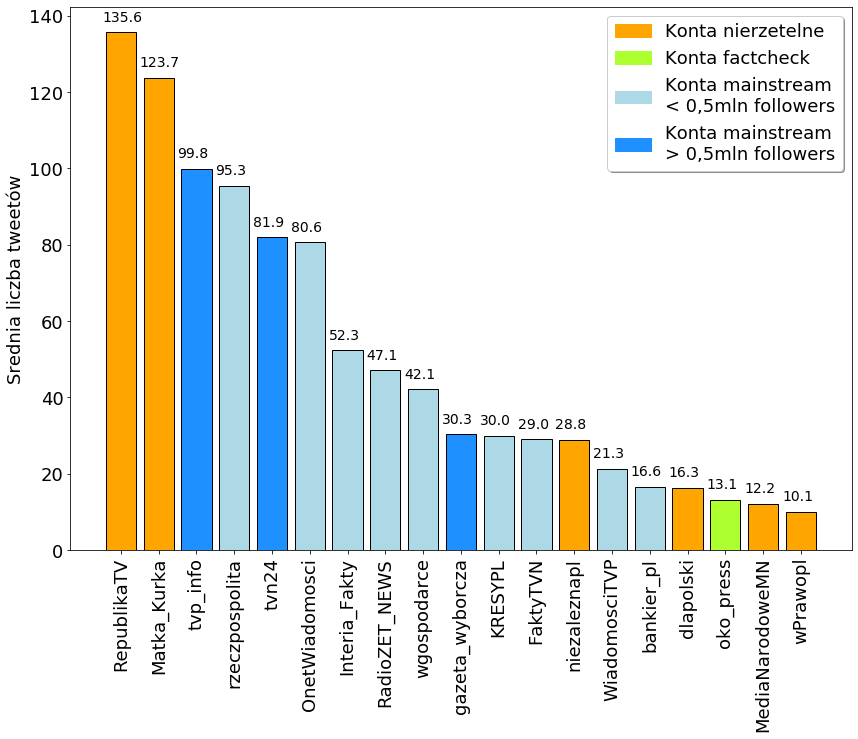
\includegraphics[width=0.9\linewidth]{img/results/tweetsperday.png}
	\caption{Wykres średniej liczby publikowanych oryginalnych tweetów na dzień dla najbardziej aktywnych kont z\,podziałem na przynależność do klasy} \label{fig:tweetsperday}
\end{figure}
\par
Badając liczbę oryginalnych tweetów dla każdego z\,kont stworzono wykres najbardziej aktywnych kont. Aktywność liczono jako średnią liczbę oryginalnych postów na dzień. Wyniki przedstawiono w\,wykresie na rysunku \ref{fig:tweetsperday}. Okazuje się, że różnica w\,aktywności kont jest ogromna. Są konta i\,z kategorii nierzetelne oraz z\,kategorii mainstream które publikują średnio po kilkaset oryginalnych postów dziennie. W\,analizowanym zbiorze znajduje się jednak też kilka kont, które są prawie nieaktywne co oznacza, że zebrano dla nich mniej niż 10 tweetów w\,badanym okresie czasu. Dodatkowo dla konta crowdmedia nie istniał żaden post możliwy do pobrania.